\section{530 --- Minimum Absolute Difference in BST}
Given a binary search tree with non-negative values, find the minimum absolute difference between values of any two nodes.

\paragraph{Example:}

\begin{flushleft}
\textbf{Input}:

\begin{figure}[H]
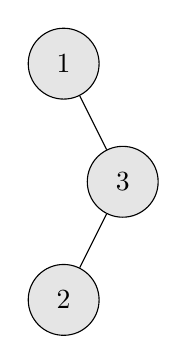
\begin{tikzpicture}
[every node/.style={draw, circle, minimum size=9mm, fill=gray!20!}]
\node{1}
	child[missing]
	child{node{3} child{node{2}} child[missing]};
\end{tikzpicture}
\end{figure}


\textbf{Output}:
1


\textbf{Explanation}:

The minimum absolute difference is 1, which is the difference between 2 and 1 (or between 2 and 3).

\end{flushleft} 

\paragraph{Note:} 
\begin{itemize}
\item There are at least two nodes in this BST.
\end{itemize}